% Copyright 2021  Stefano Fochesatto

\documentclass[xcolor={svgnames},
               hyperref={colorlinks,citecolor=DeepPink4,linkcolor=FireBrick,urlcolor=Maroon}]
               {beamer}

\mode<presentation>{
  \usetheme{Berlin}
  \usecolortheme{orchid}
  \setbeamercovered{transparent}
  \setbeamerfont{frametitle}{size=\large}
}
\usetheme[headline,footline]{UAFblue}
\setbeamercolor*{block title}{bg=red!10}
\setbeamercolor*{block body}{bg=red!5}

\usepackage[english]{babel}
\usepackage[latin1]{inputenc}
\usepackage{times}
\usepackage[T1]{fontenc}
% Or whatever. Note that the encoding and the font should match. If T1
% does not look nice, try deleting the line with the fontenc.

\usepackage{empheq,bm}
\usepackage{xspace}
\usepackage{fancyvrb}

\usepackage{tikz}
\usetikzlibrary{shapes,arrows.meta,decorations.markings,decorations.pathreplacing,fadings,positioning}

\usepackage[kw]{pseudo}
\pseudoset{left-margin=15mm,topsep=5mm,idfont=\texttt,st-left=,st-right=}


% If you wish to uncover everything in a step-wise fashion, uncomment
% the following command:
%\beamerdefaultoverlayspecification{<+->}

\newcommand{\ba}{\mathbf{a}}
\newcommand{\bb}{\mathbf{b}}
\newcommand{\bc}{\mathbf{c}}
\newcommand{\bbf}{\mathbf{f}}
\newcommand{\bg}{\mathbf{g}}
\newcommand{\bn}{\mathbf{n}}
\newcommand{\bq}{\mathbf{q}}
\newcommand{\br}{\mathbf{r}}
\newcommand{\bx}{\mathbf{x}}
\newcommand{\by}{\mathbf{y}}
\newcommand{\bv}{\mathbf{v}}
\newcommand{\bu}{\mathbf{u}}
\newcommand{\bw}{\mathbf{w}}

\usepackage{tikz}



\newcommand{\bF}{\mathbf{F}}
\newcommand{\bG}{\mathbf{G}}
\newcommand{\bQ}{\mathbf{Q}}

\newcommand{\grad}{\nabla}
\newcommand{\Div}{\nabla\cdot}
\newcommand{\minmod}{\operatorname{minmod}}

\newcommand{\CC}{\mathbb{C}}
\newcommand{\RR}{\mathbb{R}}

\newcommand{\ddt}[1]{\ensuremath{\frac{\partial #1}{\partial t}}}
\newcommand{\ddx}[1]{\ensuremath{\frac{\partial #1}{\partial x}}}
\newcommand{\Matlab}{\textsc{Matlab}\xspace}
\newcommand{\Octave}{\textsc{Octave}\xspace}
\newcommand{\eps}{\epsilon}

\newcommand{\ip}[2]{\left<#1,#2\right>}

\newcommand{\xiphalf}{{x_{i+\frac{1}{2}}}}
\newcommand{\ximhalf}{{x_{i-\frac{1}{2}}}}
\newcommand{\Fiphalf}{{F_{i+\frac{1}{2}}}}
\newcommand{\Fimhalf}{{F_{i-\frac{1}{2}}}}
\newcommand{\Fiphalfn}{{F^n_{i+\frac{1}{2}}}}
\newcommand{\Fimhalfn}{{F^n_{i-\frac{1}{2}}}}

\newcommand{\trefcolumn}[1]{\begin{bmatrix} \phantom{x} \\ #1 \\ \phantom{x} \end{bmatrix}}
\newcommand{\trefmatrixtwo}[2]{\left[\begin{array}{c|c|c} & & \\ #1 & \dots & #2 \\ & & \end{array}\right]}
\newcommand{\trefmatrixthree}[3]{\left[\begin{array}{c|c|c|c} & & & \\ #1 & #2 & \dots & #3 \\ & & & \end{array}\right]}
\newcommand{\trefmatrixgroups}[4]{\left[\begin{array}{c|c|c|c|c|c} & & & & & \\ #1 & \dots & #2 & #3 & \dots & #4 \\ & & & & & \end{array}\right]}

\newcommand{\blocktwo}[4]{\left[\begin{array}{c|c} #1 & #2 \\ \hline #3 & #4 \end{array}\right]}

\newcommand{\bqed}{{\color{blue}\qed}}
\newcommand{\ds}{\displaystyle}

\newcommand\mynum[1]{{\renewcommand{\insertenumlabel}{#1}%
      \usebeamertemplate{enumerate item} \,}}


\title{Decision Tree Learning from Scratch}

\author{Stefano Fochesatto}

\institute[UAF]{MATH 692 Mathematics for Machine Learning}

\date[Spring 2022]{2/10/2022}

%\titlegraphic{\begin{picture}(0,0)
%    \put(0,180){\makebox(0,0)[rt]{\includegraphics[width=4cm]{figs/software.png}}}
%  \end{picture}
%}

%% this nonsense needed to start section counter at 0; see
%% https://tex.stackexchange.com/questions/170222/change-the-numbering-in-beamers-table-of-content
\makeatletter
\patchcmd{\beamer@sectionintoc}
  {\ifnum\beamer@tempcount>0}
  {\ifnum\beamer@tempcount>-1}
  {}
  {}
%\beamer@tocsectionnumber=-1
\makeatother


\begin{document}
\beamertemplatenavigationsymbolsempty

\begin{frame}
  \maketitle
\end{frame}

\begin{frame}{Presentation Outline}
  \begin{itemize}
  \item What is a Decision Tree?
  \vfill
  \item Training the Tree.
  \vfill
  \item Code Demo.
  \vfill
  \item Advantages and Pitfalls.
  \vfill
  \item Application in Ensemble Models.
  \end{itemize}
\end{frame}







\begin{frame}{What is Decision Tree?}
    \begin{columns}[T]
      \begin{column}{.60\textwidth}
        \begin{center}
        \begin{itemize}
            \item Supervised Learning.  
            \item A flowchart where internal nodes represent a test for the data.
            \item Leaf nodes apply classification label or regression.
            \item Derived from recursive partitioning. 
            \item All nodes represent some partition of the data.
            \item We will discuss classification mainly, 
        \end{itemize}
      \end{center}
      \end{column}
      \begin{column}{.50\textwidth}
            \begin{figure}
              \vspace*{\fill}
              \begin{center}
            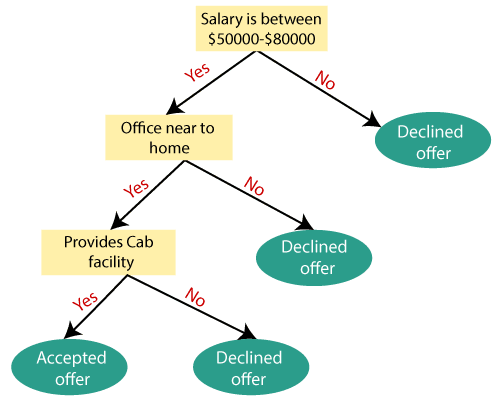
\includegraphics[width=.75\textwidth]{ExampleTree.png}
          \caption{Decision Tree Example}
              \end{center}
              \vspace*{\fill}
            \end{figure}
          \end{column}
    \end{columns}
  \end{frame}

  \begin{frame}{What is Decision Tree?}
            \begin{figure}
              \vspace*{\fill}
              \begin{center}
            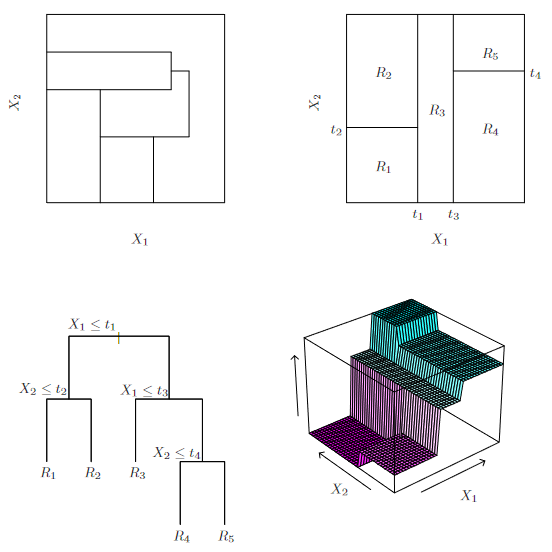
\includegraphics[width=.55\textwidth]{ESLDecisionTreeExample.png}
          \caption{E.S.L. Friedman, Hastie, Tibshirani}
              \end{center}
              \vspace*{\fill}
            \end{figure}
  \end{frame}


  \begin{frame}{What is Decision Tree?}
  \begin{itemize}
    \item Small Demo building a decision tree. 
  \end{itemize}
  \end{frame}





  
  \begin{frame}{Training the Tree.}
    \begin{itemize}
    \item Methods don't guarantee the optimal solution (Greedy). 
    \vfill
    \item Top-Down Induction of Decision Trees (R.Quinlan)
    \vfill
    \item There are several algorithms for training.
      \begin{itemize}
        \item CART (L.Breimann et al., 1984)
        \item ID3 and C4.5 (R.Quinlan 1983, 93)
        \item C5.0 (R.Quinlan)
        \item and many more...
      \end{itemize}
    \end{itemize}

  \end{frame}

  
  \begin{frame}{Information Theory}
    \begin{itemize}
      \item Consider the following splits,
      \begin{columns}[T]
        \begin{column}{.45\textwidth}
          \begin{figure}
            \vspace*{\fill}
            \begin{center}
          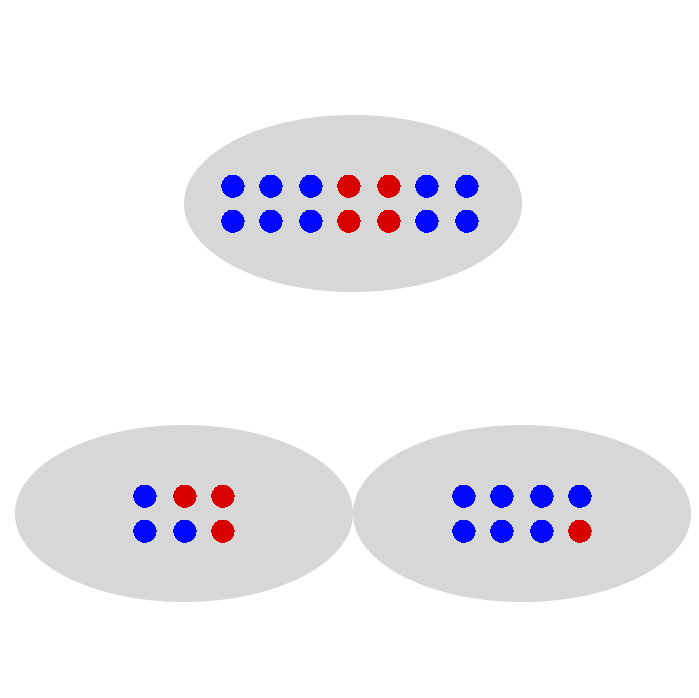
\includegraphics[width=.85\textwidth]{HighEntropy.png}
        \caption{Example Split \# 1}
            \end{center}
            \vspace*{\fill}
          \end{figure}
        \end{column}
        \begin{column}{.45\textwidth}
              \begin{figure}
                \vspace*{\fill}
                \begin{center}
              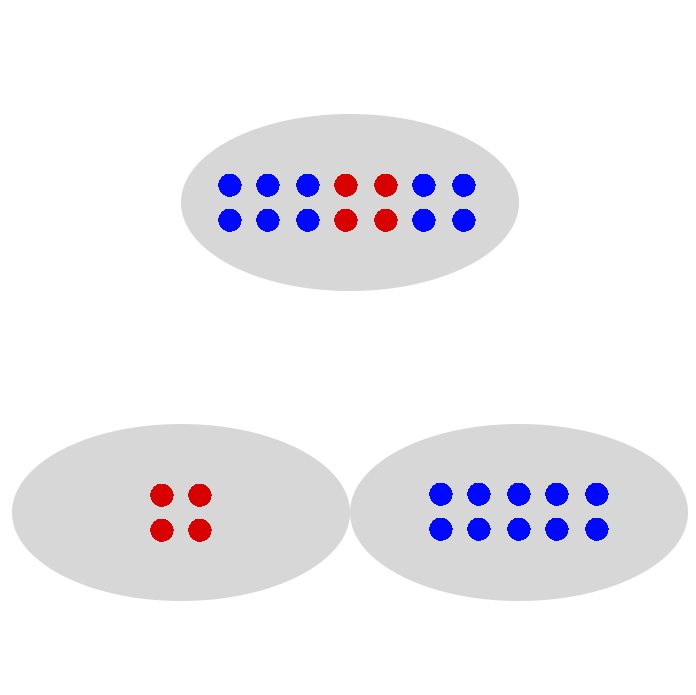
\includegraphics[width=.85\textwidth]{LowEntropy.png}
            \caption{Example Split \# 2}
                \end{center}
                \vspace*{\fill}
              \end{figure}
            \end{column}
      \end{columns}
      \item To optimize our tree we need to be able to quantify the quality of a split (or generalized node)?
    \end{itemize}  
  \end{frame}


  \begin{frame}{Information Theory}
      \begin{columns}[T]
        \begin{column}{.60\textwidth}
          \begin{itemize}
            \item Let $X$ be a discrete random variable which represents a node $S$'s predicted class. 
            \vfill
            \item Let $p(x)$ be the probability mass function.
            \vfill
            \item Consider the following example,
            \begin{equation*}
              p(\tikz\draw[red,fill=red] (0,0) circle (.5ex);) = \dfrac{\text{$\#$ of \tikz\draw[red,fill=red] (0,0) circle (.5ex);}}{\text{Total $\#$ data in $S$}} = \dfrac{3}{5}, 
            \end{equation*}
            \begin{equation*}
              p(\tikz\draw[blue,fill=blue] (0,0) circle (.5ex);) = \dfrac{\text{$\#$ of \tikz\draw[blue,fill=blue] (0,0) circle (.5ex);}}{\text{Total $\#$ data in $S$}} = \dfrac{2}{5}. 
            \end{equation*}
          \end{itemize}
        \end{column}
        \begin{column}{.40\textwidth}
          \begin{figure}
            \vspace*{\fill}
            \begin{center}
          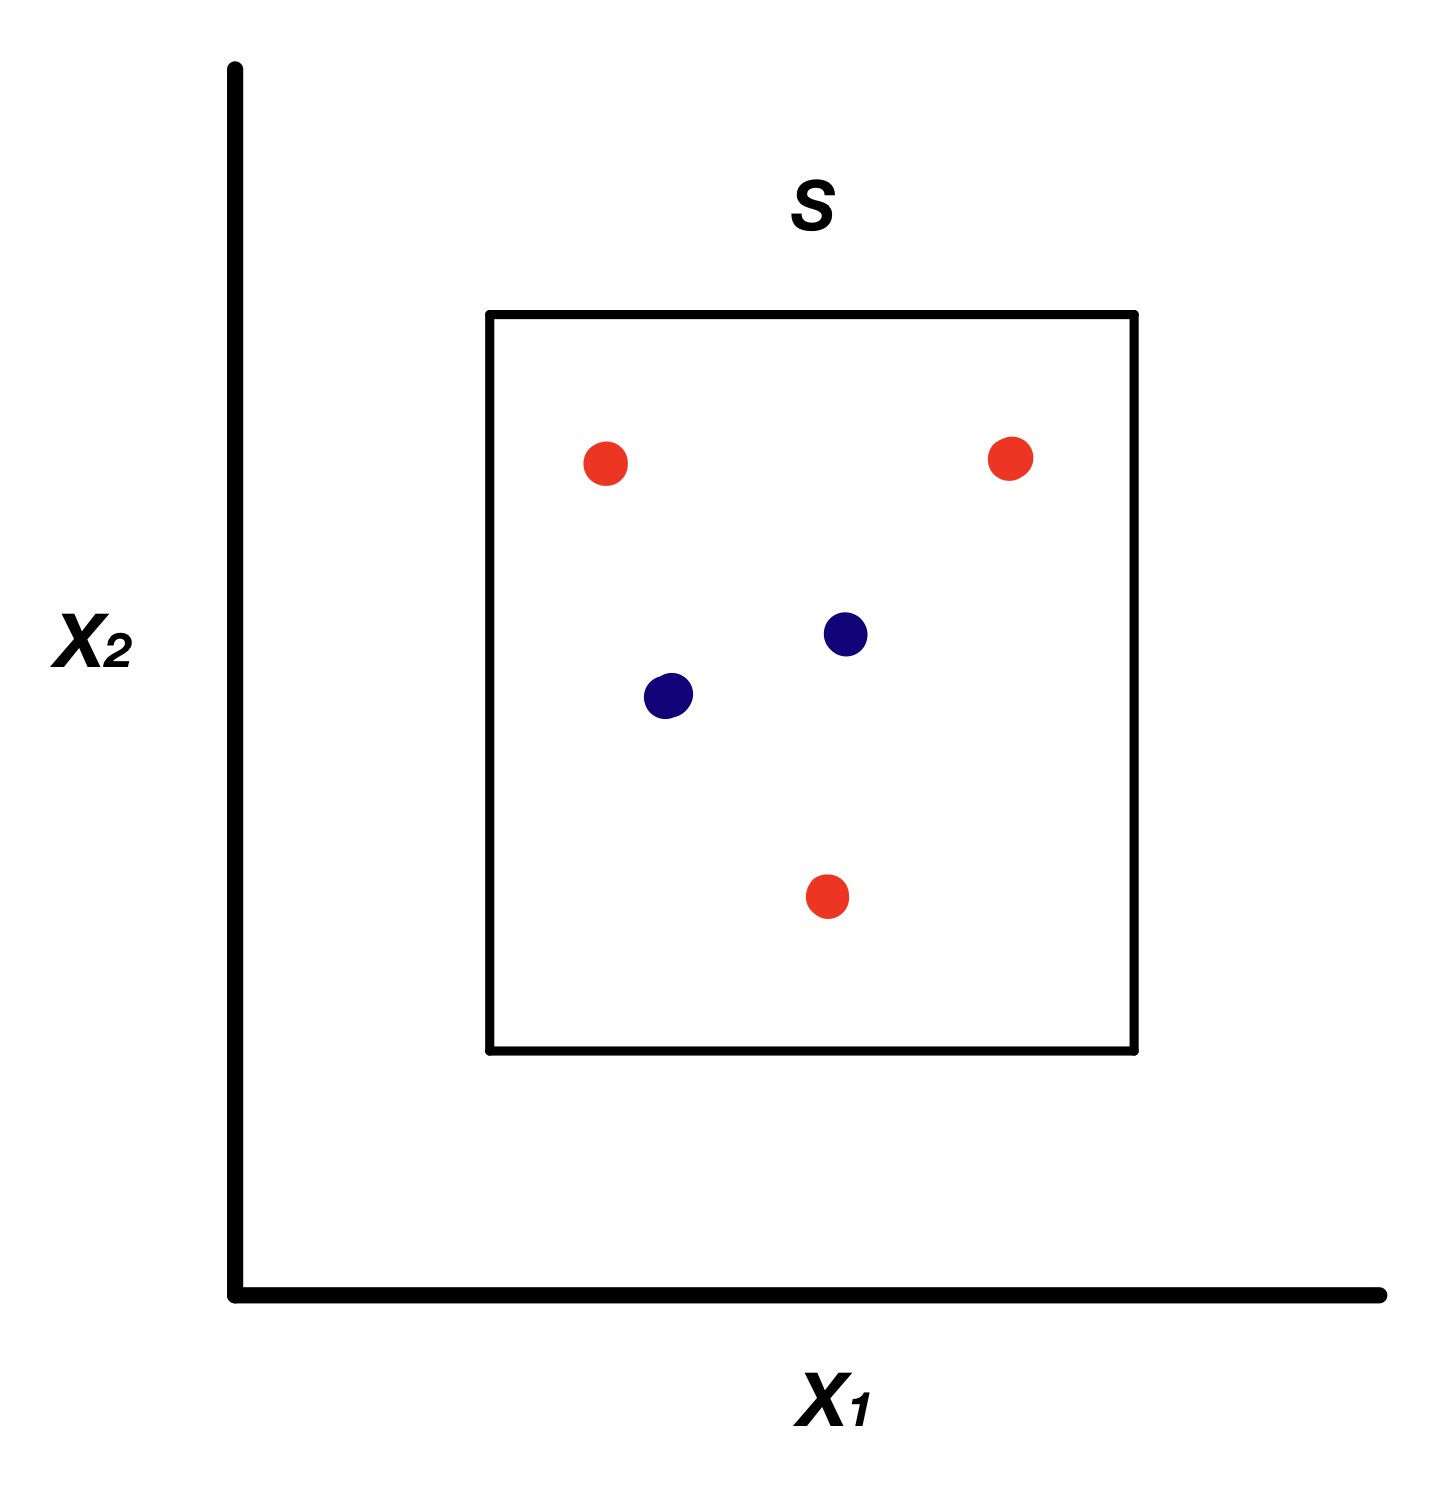
\includegraphics[width=\textwidth]{NodeS.jpg}
            \end{center}
            \vspace*{\fill}
          \end{figure}
        \end{column}
      \end{columns}
  \end{frame}











  \begin{frame}{Information Theory}
    \begin{itemize}
      \item From the previous slide we know that $X$ is a d.r.v with $n$(classes) possible outcomes and pmf $p(x)$. Now consider the following,
      \vfill
      \item In information theory, the unit of information ascribed to an outcome $x \in [n]$ is a log measure of 1/p(x),
      \begin{equation*}
        I = \log_2\left(\frac{1}{p(x)}\right) = -\log_2(p(x)).
      \end{equation*} 
      \vfill
      \item Events that are rare have more information, events that are common have less information. 
    \end{itemize}
  \end{frame}

  \begin{frame}{Information Theory}
    \begin{itemize}
      \item We want to know the expected information at a node over all outcomes (classification classes), 
      \begin{equation*}
        \mathbb{E}(I) = \sum_{i = 1}^n p(i) \log_2\left(\frac{1}{p(i)}\right) = -\sum_{i = 1}^n p(i)\log_2(p(i)).
      \end{equation*}
      \vfill
      \item We want to find the split which maximizes $\Delta I$ or information gain, 
      \begin{equation*}
        \Delta I = \mathbb{E}(I)_{Parent} - \sum w(i) \mathbb{E}(I)_{Children}.  
      \end{equation*}
      \item Where $w(i)$ is the size of the child node relative to the parent node. 
      \vfill
      \item Sometimes we only care about the difference between splits. 
      \begin{equation*}
        \Delta I = 1 - \sum w(i) \mathbb{E}(I)_{Children}.  
      \end{equation*}
    \end{itemize}
  \end{frame}


  \begin{frame}{Training the Tree}
    \begin{itemize}
    \item For the CART algorithm the Gini Impurity is used to evaluate the quality of a node, 
    \begin{equation*}
      Gini = 1 - \sum_{i = 1}^n p(i)^2.
    \end{equation*}
    \item Again evaluating a split we take a weighted sum, 
    \begin{equation*}
      Gini_{split} = \sum w(i) Gini_{children}.
    \end{equation*}
    \item Both methods are largely the same, Gini is preferred for predictive performance and computational complexity. 
  \end{itemize}
  \end{frame}


  \begin{frame}{Training the Tree}
    \begin{figure}
      \vspace*{\fill}
      \begin{center}
    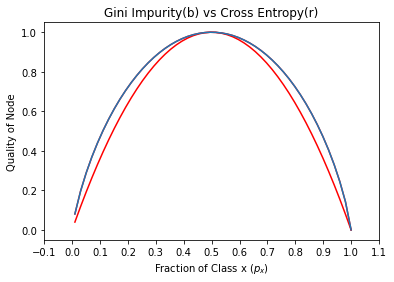
\includegraphics[width=.75\textwidth]{GinivsCrossEntropy.png}
      \end{center}
      \vspace*{\fill}
    \end{figure}
  \end{frame}

  


  \begin{frame}{Training the Tree}
    \begin{itemize}
      \item A Very Naive Algorithm:
      \begin{itemize}
        \item Search through each feature, threshold pair to find the optimal split for the current partition. 
        \item Partition the data.
        \item Recurse.
        \item Exit through hyperparameter or complete classification of training data.
      \end{itemize}
      \vfill
      \item Code Demo
    \end{itemize}
  \end{frame}


  \begin{frame}{Advantages and Pitfalls.}
    \begin{itemize}
      \item Mimics human decision making. 
      \vfill
      \item Can handle numerical and categorical data.
      \vfill
      \item Is an open-box model.
      \vfill
      \item Has naive runtime of $O(mn^2log(n))$. 
      \vfill
      \item It is robust to colinearity.
      \vfill
      \item Built-in metric for feature importance (with caveats)
      \vfill
      \item Very robust when boosted and bagged.
    \end{itemize}
  \end{frame}


  \begin{frame}{Advantages and Pitfalls.}
    \begin{itemize}
      \item Will be easily outperformed by other methods against linear decision boundaries,
      \begin{figure}
        \vspace*{\fill}
        \begin{center}
      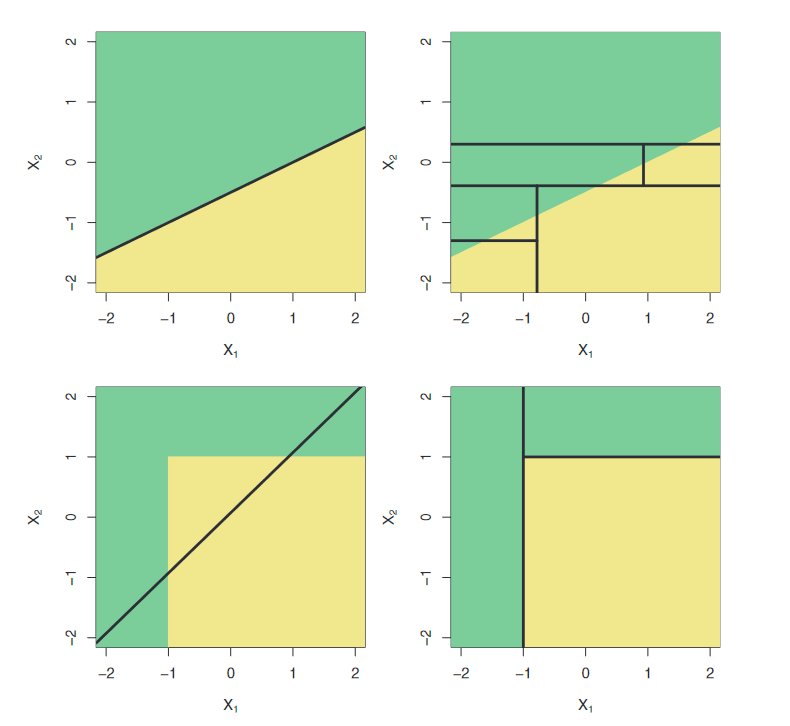
\includegraphics[width=.50\textwidth]{LinearBoudary.png}
        \end{center}
        \caption{I.S.L. James, Witten, Hastie, Tibshirani}
        \vspace*{\fill}
      \end{figure}
    \end{itemize}
  \end{frame}

  
  \begin{frame}{Advantages and Pitfalls.}
    \begin{itemize}
      \item Is prone to overfitting, 
      \begin{figure}
        \vspace*{\fill}
        \begin{center}
      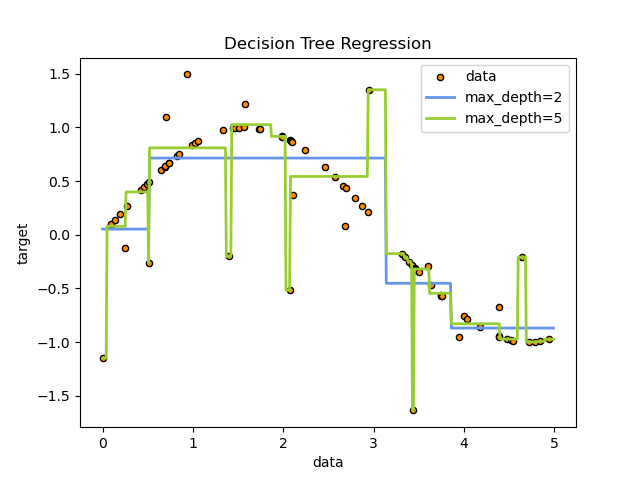
\includegraphics[width=.70\textwidth]{Overfitting.png}
        \end{center}
        \caption{SKLearn Docs}
        \vspace*{\fill}
      \end{figure}
    \end{itemize}
  \end{frame}




  \begin{frame}{Dealing with Overfitting.}
    \begin{itemize}
      \item Generally there are two ways to deal with overfitting.
        \begin{itemize}
          \item Tuning Hyperparameters (pre-pruning)
       
          \begin{itemize}
            \item max depth, min samples leaf, min samples split\dots
            \item Grid Search Optimization =(
          \end{itemize}
          \vfill
          
          \item Cost Complexity Analysis (post-pruning)
          \begin{itemize}
            \item Another optimization problem.
            \item Grow Tree $T_0$ to Maximal Length,
            \item Find the sub tree $T \subset T_0$ which minimizes the following, 
            \begin{equation*}
              C(T)_{\alpha} = \sum_{Internal Nodes}^{|T|} Entropy + \alpha|T|
            \end{equation*}
            \item $\alpha$ is another parameter which is estimated using cross-validation. 
          \end{itemize}
        \end{itemize}
      
        \item Note the Bias-Variance trade-off of pruning. 
    \end{itemize}
  \end{frame}



  \begin{frame}{Applications in Ensemble Models.}
    \begin{itemize}
      \item Bagging (and RandomForest)
        \begin{itemize}
          \item The underlying idea is model averaging (many to one).
          \item Bootstrap the data (RandomForest means bootstrapping features). 
          \item Construct several full size decision trees.
          \item When predicting average the results (majority vote).  
        \end{itemize}
        \vfill
      \item Individual models have very low bias.
      \item Averaging the models reduces the variance.
    \end{itemize}
  \end{frame}


  \begin{frame}{Applications in Ensemble Models.}
    \begin{itemize}
      \item Decision Tree Ensembles are good.
      \begin{figure}
        \vspace*{\fill}
        \begin{center}
      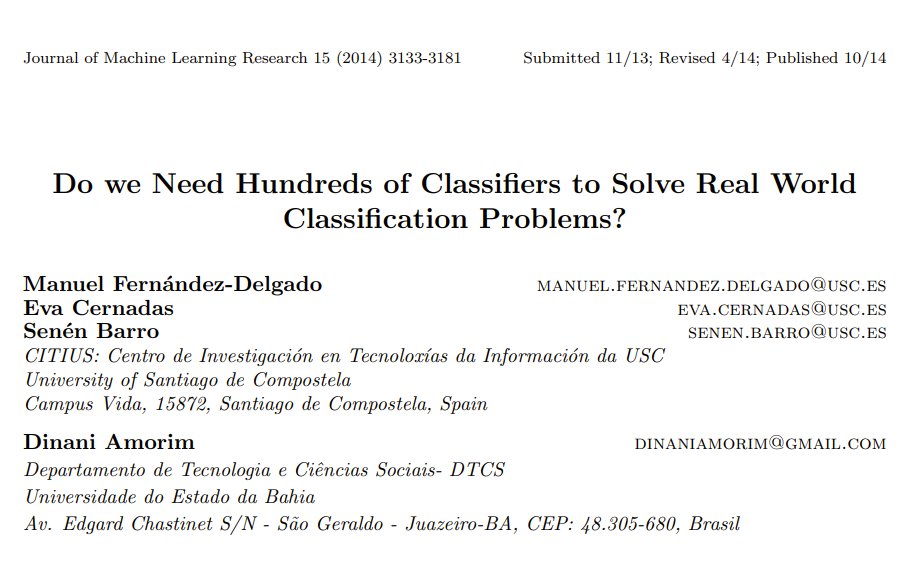
\includegraphics[width=.50\textwidth]{Delgado.png}
        \end{center}
        \caption{179 Classifiers, 17 families, 121 datasets}
        \vspace*{\fill}
      \end{figure}
      
      
      \item Concluded that the best classifier over several datasets and metrics was an implementation of RandomForest.
      \item Six RandomForest classifiers and five SVM were among the top 20 classifiers. 

    \end{itemize}
  \end{frame}


  
  \begin{frame}{Applications in Ensemble Models.}
    \begin{itemize}
      \item Decision Tree Ensembles are good. 
      \begin{figure}
        \vspace*{\fill}
        \begin{center}
      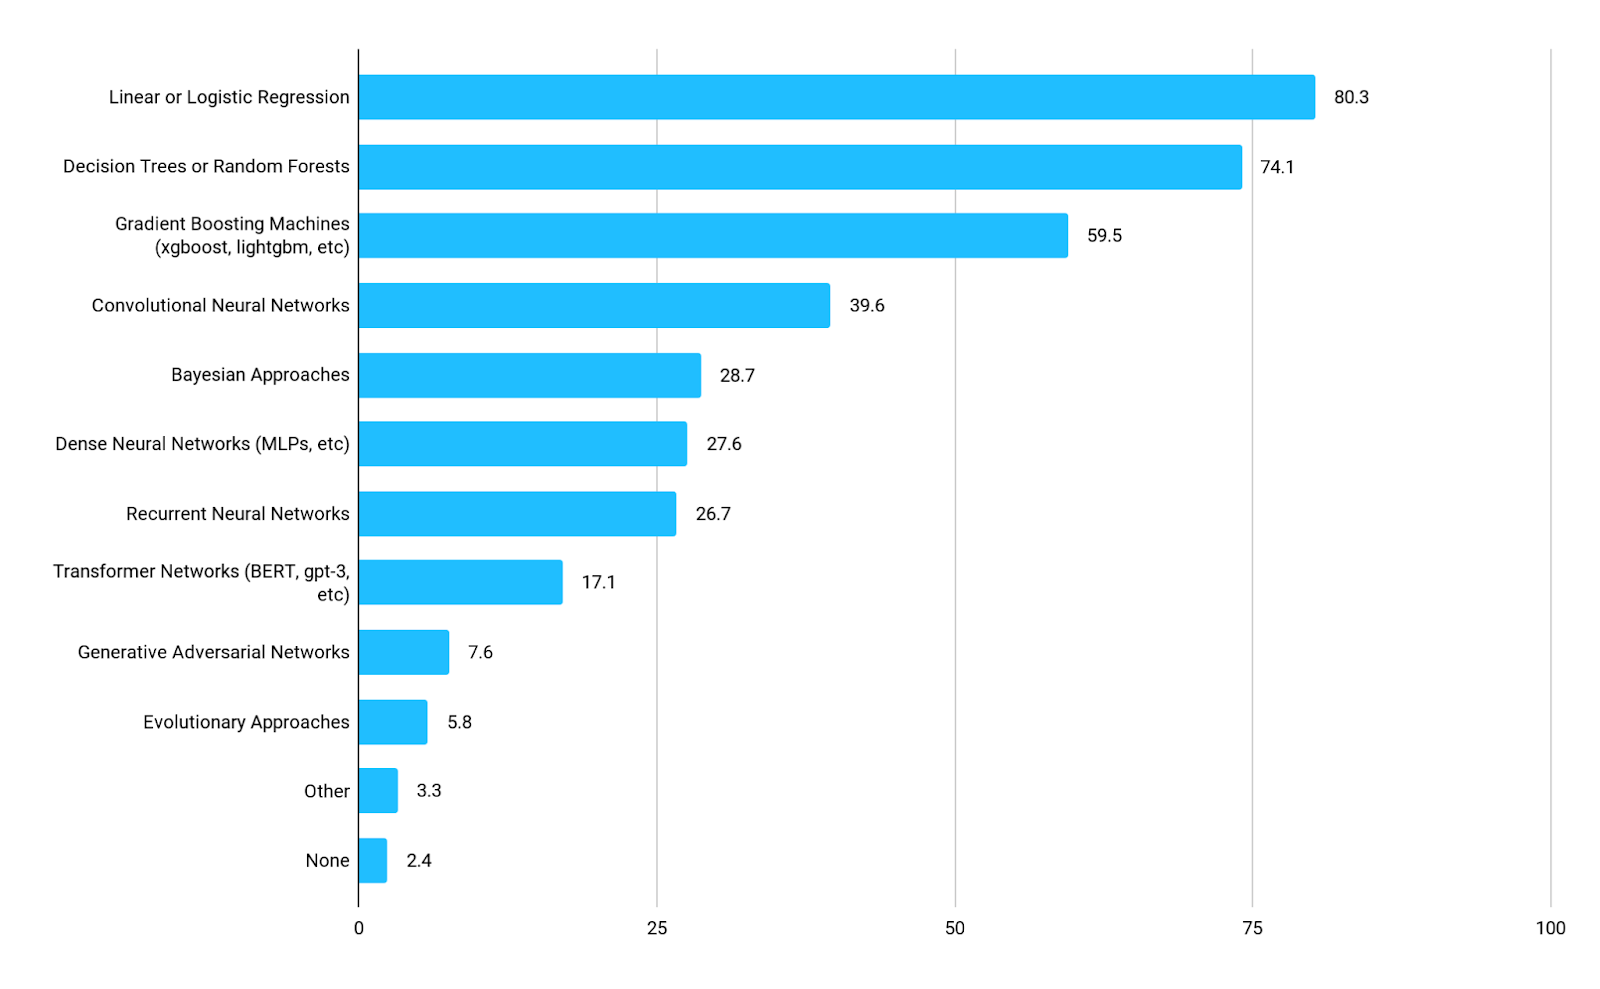
\includegraphics[width=.65\textwidth]{Kaggle.png}
        \end{center}
        \caption{2021 Kaggle survery: Over 25,000 Data Scientists and ML Engineers.}
        \vspace*{\fill}
      \end{figure}
      \item Among ML practitioners decision trees are nearly as ubiquitous as regression.  
    \end{itemize}
  \end{frame}


  






\end{document}